% =============================================================================
%  Báo cáo trình chiếu — da2: Triển khai mô hình SVM chẩn đoán ung thư vú
%  Biên dịch:  latexmk -xelatex da2_slide.tex   (Overleaf: Compiler = XeLaTeX)
%  Số liệu: macro trong metrics_data.tex, sinh bằng python docs/latex/make_tex_data.py
% =============================================================================
\documentclass[aspectratio=169,12pt]{beamer}

\usetheme{Madrid}
\usecolortheme{whale}
\setbeamertemplate{navigation symbols}{}
\setbeamertemplate{caption}{\insertcaption}
\setbeamerfont{block title}{size=\normalsize}

\usepackage{fontspec}
\setmainfont{Latin Modern Roman}
\setsansfont{Latin Modern Sans}
\setmonofont{DejaVu Sans Mono}[Scale=0.78]

\usepackage[vietnamese]{babel}
\usepackage{amsmath,amssymb}
\usepackage{graphicx}
\usepackage{booktabs}
\usepackage{listings}
\usepackage{xcolor}
\usepackage{tikz}
\usetikzlibrary{positioning,arrows.meta}

\graphicspath{{../../reports/figures/}{../screenshots/}{./}}

% Địa chỉ dịch vụ trên Render: đổi bằng  python docs/latex/set_service_url.py <URL mới>

\definecolor{rose}{HTML}{C2255C}
\definecolor{warnbg}{HTML}{FFF4E5}
\setbeamercolor{alerted text}{fg=rose}
\definecolor{codebg}{HTML}{F5F5FA}
\lstset{
  backgroundcolor=\color{codebg},
  basicstyle=\ttfamily\scriptsize,
  keywordstyle=\color{blue!70!black}\bfseries,
  stringstyle=\color{teal},
  commentstyle=\color{gray}\itshape,
  breaklines=true, showstringspaces=false,
  frame=single, rulecolor=\color{gray!40},
  extendedchars=true, inputencoding=utf8,
}

% Tệp sinh tự động bởi docs/latex/make_tex_data.py — KHÔNG sửa tay.
% Nguồn: reports/metrics.json + artifacts/metadata.json (train lúc 2026-09-26T12:35:51+00:00)

\newcommand{\GeneratedAt}{2026-09-26 12:35:51 U C}
\newcommand{\ModelName}{\texttt{breast-cancer-svm-rbf}}
\newcommand{\ModelVersion}{1.0.0}
\newcommand{\SklearnVersion}{1.9.1}
\newcommand{\NumpyVersion}{2.5.3}
\newcommand{\PythonVersion}{3.12.10}
\newcommand{\DataHashShort}{25e2eb7b7a87}
\newcommand{\NSamples}{569}
\newcommand{\NFeatures}{30}
\newcommand{\NMalignant}{212}
\newcommand{\NBenign}{357}
\newcommand{\PctMalignant}{37.3\%}
\newcommand{\PctBenign}{62.7\%}
\newcommand{\NTrain}{455}
\newcommand{\NTest}{114}
\newcommand{\TestMalignant}{42}
\newcommand{\TestBenign}{72}
\newcommand{\NZeroRows}{13}
\newcommand{\NZeroFeatures}{6}
\newcommand{\ZeroFeatures}{\texttt{mean concavity}, \texttt{mean concave points}, \texttt{concavity error}, \texttt{concave points error}, \texttt{worst concavity}, \texttt{worst concave points}}
\newcommand{\RandomState}{42}
\newcommand{\UpperFactor}{3}
\newcommand{\PcaOne}{44.3\%}
\newcommand{\PcaTwo}{19.0\%}
\newcommand{\PcaTotal}{63.2\%}
\newcommand{\GridConfigs}{16}
\newcommand{\GridSeconds}{2.8}
\newcommand{\GridScoring}{\texttt{recall\_macro}}
\newcommand{\BestC}{10}
\newcommand{\BestGamma}{0.01}
\newcommand{\GridCVMean}{0.9753}
\newcommand{\GridCVStd}{0.0162}
\newcommand{\CalibChosen}{\texttt{calibrated\_sigmoid\_single}}
\newcommand{\CalibChosenBrier}{0.01903}
\newcommand{\CalibBaselineBrier}{0.01873}
\newcommand{\CalibSigmoidBrier}{0.02476}
\newcommand{\CalibIsotonicBrier}{0.01956}
\newcommand{\Threshold}{0.3993}
\newcommand{\TargetSens}{0.97}
\newcommand{\ImpliedCostRatio}{1.50}
\newcommand{\TrainSens}{0.9824}
\newcommand{\TrainSpec}{0.9895}
\newcommand{\CVSens}{0.9706}
\newcommand{\CVSpec}{0.9789}
\newcommand{\CVTP}{165}
\newcommand{\CVFN}{5}
\newcommand{\CVFP}{6}
\newcommand{\CVHalfSens}{0.9647}
\newcommand{\CVHalfSpec}{0.9860}
\newcommand{\CVHalfTP}{164}
\newcommand{\CVHalfFN}{6}
\newcommand{\CVHalfFP}{4}
\newcommand{\CVMalignant}{170}
\newcommand{\TestSens}{0.9762}
\newcommand{\TestSpec}{0.9306}
\newcommand{\TestPrec}{0.8913}
\newcommand{\TestFOne}{0.9318}
\newcommand{\TestNPV}{0.9853}
\newcommand{\TestAcc}{0.9474}
\newcommand{\TestAUC}{0.9967}
\newcommand{\TestPRAUC}{0.9952}
\newcommand{\TestBrier}{0.0235}
\newcommand{\TestTP}{41}
\newcommand{\TestFN}{1}
\newcommand{\TestFP}{5}
\newcommand{\TestTN}{67}
\newcommand{\HalfSens}{0.9762}
\newcommand{\HalfSpec}{0.9722}
\newcommand{\HalfPrec}{0.9535}
\newcommand{\HalfFN}{1}
\newcommand{\HalfFP}{2}
\newcommand{\TestNErrors}{6}
\newcommand{\MissedProba}{0.0987}
\newcommand{\FPMinProba}{0.4617}
\newcommand{\FPMaxProba}{0.7249}
\newcommand{\FPBelowHalf}{3}

% Bảng so sánh cách hiệu chỉnh xác suất (4 cột)
\newcommand{\CalibRows}{%
  \texttt{svc\_probability} & 0.01873 & 0.07208 & 0.9958 & Platt trong libsvm, deprecated từ 1.9 \\
  \textbf{\texttt{calibrated\_sigmoid\_single}} & 0.01903 & 0.07381 & 0.9955 & khuyến nghị thay \texttt{probability=True} \\
  \texttt{calibrated\_sigmoid} & 0.02476 & 0.10639 & 0.9959 & trung bình 5 mô hình đã hiệu chỉnh \\
  \texttt{calibrated\_isotonic} & 0.01956 & 0.13740 & 0.9937 & hồi quy đơn điệu, không tham số \\
}

% Bảng metric train / CV / test (10 cột)
\newcommand{\MetricRows}{%
  Train & 0.3993 & 0.9824 & 0.9895 & 0.9824 & 0.9824 & 0.9983 & 0.9978 & 3 & 3 \\
  CV out-of-fold & 0.3993 & 0.9706 & 0.9789 & 0.9649 & 0.9677 & 0.9955 & 0.9946 & 5 & 6 \\
  \textbf{Test} & 0.3993 & 0.9762 & 0.9306 & 0.8913 & 0.9318 & 0.9967 & 0.9952 & 1 & 5 \\
  Test, ngưỡng 0.5 & 0.5000 & 0.9762 & 0.9722 & 0.9535 & 0.9647 & 0.9967 & 0.9952 & 1 & 2 \\
}

% Bảng metric rút gọn cho slide (6 cột)
\newcommand{\MetricRowsShort}{%
  Train & 0.9824 & 0.9895 & 0.9824 & 0.9983 & 3 \\
  CV (OOF) & 0.9706 & 0.9789 & 0.9649 & 0.9955 & 5 \\
  \textbf{Test} & 0.9762 & 0.9306 & 0.8913 & 0.9967 & 1 \\
  Test @ 0.5 & 0.9762 & 0.9722 & 0.9535 & 0.9967 & 1 \\
}

% Các mẫu test bị dự đoán sai (4 cột)
\newcommand{\ErrorRows}{%
  3 & lành tính & ác tính & 0.4617 \\
  16 & lành tính & ác tính & 0.7249 \\
  38 & lành tính & ác tính & 0.4707 \\
  51 & lành tính & ác tính & 0.4932 \\
  53 & ác tính & lành tính & 0.0987 \\
  66 & lành tính & ác tính & 0.5096 \\
}

% Kết quả GridSearchCV (4 cột)
\newcommand{\GridRows}{%
  10 & 0.01 & 0.9753 $\pm$ 0.0162 & 1 \\
  10 & 0.001 & 0.9736 $\pm$ 0.0059 & 2 \\
  1 & scale & 0.9730 $\pm$ 0.0107 & 3 \\
  1 & 0.01 & 0.9724 $\pm$ 0.0080 & 4 \\
  100 & 0.001 & 0.9724 $\pm$ 0.0080 & 4 \\
  100 & scale & 0.9666 $\pm$ 0.0232 & 6 \\
  10 & scale & 0.9654 $\pm$ 0.0089 & 7 \\
  1 & 0.1 & 0.9578 $\pm$ 0.0132 & 8 \\
  100 & 0.01 & 0.9577 $\pm$ 0.0133 & 9 \\
  10 & 0.1 & 0.9461 $\pm$ 0.0249 & 10 \\
  100 & 0.1 & 0.9461 $\pm$ 0.0249 & 10 \\
  0.1 & scale & 0.9449 $\pm$ 0.0121 & 12 \\
  1 & 0.001 & 0.9371 $\pm$ 0.0207 & 13 \\
  0.1 & 0.01 & 0.9330 $\pm$ 0.0206 & 14 \\
  0.1 & 0.1 & 0.9081 $\pm$ 0.0313 & 15 \\
  0.1 & 0.001 & 0.8624 $\pm$ 0.0428 & 16 \\
}

% ----- So sánh 5 mô hình phân loại (reports/comparison.json, train lúc 2026-09-27T06:34:11+00:00) -----
\newcommand{\CmpNModels}{5}
\newcommand{\CmpSeconds}{17.1}
\newcommand{\CmpBestLabel}{Logistic Regression}
\newcommand{\CmpBestCV}{0.9760}
\newcommand{\CmpBestCVStd}{0.0116}
\newcommand{\CmpSvmCV}{0.9753}
\newcommand{\CmpSvmCVStd}{0.0162}
\newcommand{\CmpGap}{0.0007}
\newcommand{\CmpBestSpec}{0.9861}
\newcommand{\CmpFastestLabel}{Logistic Regression}
\newcommand{\CmpFastestUs}{4.3}
\newcommand{\CmpSpeedFast}{1.5}
\newcommand{\CmpSpeedMedium}{3}

% Bảng so sánh (9 cột), dòng in đậm là mô hình có CV cao nhất
\newcommand{\CmpRows}{%
  \textbf{Logistic Regression} & 0.9760 & 0.9762 & 0.9861 & 0.9954 & 0.5783 & 1/1 & 9.7 & 4.3 \\
  SVM (RBF) & 0.9753 & 0.9762 & 0.9306 & 0.9967 & 0.3993 & 1/5 & 45.9 & 21.7 \\
  SVM tuyến tính & 0.9724 & 0.9762 & 0.9444 & 0.9960 & 0.3920 & 1/4 & 47.8 & 19.0 \\
  Random Forest & 0.9613 & 0.9524 & 0.9444 & 0.9945 & 0.4900 & 2/4 & 153.5 & 82.4 \\
  K láng giềng gần (KNN) & 0.9577 & 0.9762 & 0.8889 & 0.9944 & 0.3333 & 1/8 & 1.9 & 53.5 \\
}

% Bảng rút gọn cho slide (5 cột)
\newcommand{\CmpRowsShort}{%
  \textbf{Logistic Regression} & 0.9760 & 0.9762 & 0.9861 & 0.9954 \\
  SVM (RBF) & 0.9753 & 0.9762 & 0.9306 & 0.9967 \\
  SVM tuyến tính & 0.9724 & 0.9762 & 0.9444 & 0.9960 \\
  Random Forest & 0.9613 & 0.9524 & 0.9444 & 0.9945 \\
  K láng giềng gần (KNN) & 0.9577 & 0.9762 & 0.8889 & 0.9944 \\
}



\newcommand{\canhbao}{%
  \colorbox{warnbg}{\parbox{0.96\textwidth}{\small\textbf{Chỉ phục vụ mục đích giáo dục} --- không thay thế
  bác sĩ, xét nghiệm đã thẩm định hay chẩn đoán y khoa.}}}

\title[SVM chẩn đoán ung thư vú]{Triển khai mô hình SVM\\chẩn đoán ung thư vú}
\subtitle{Breast Cancer Wisconsin · FastAPI · Render}
\author{La Thị Mỹ Hoà}
\institute{Lớp 24CKDL \\ Học phần: Học máy nâng cao}
\date{}

\begin{document}

\begin{frame}[plain]
  \titlepage
  \begin{center}\small
    \texttt{https://breast-cancer-svm-api-f2qq.onrender.com}
  \end{center}
\end{frame}

\begin{frame}{Nội dung}
  \tableofcontents
\end{frame}

% =============================================================================
\section{Bài toán và dữ liệu}
% =============================================================================

\begin{frame}{Bài toán và phạm vi sử dụng}
  \begin{columns}[T]
    \begin{column}{0.55\textwidth}
      \textbf{Đầu vào:} \NFeatures{} đặc trưng hình thái nhân tế bào, đo trên ảnh chọc hút kim nhỏ (FNA)
      \vspace{6pt}

      \textbf{Đầu ra:} khối u \alert{ác tính} hay lành tính, kèm xác suất
      \vspace{6pt}

      \textbf{Điểm khác biệt:} hai loại sai không ngang nhau --- bỏ sót ca ác tính nguy hiểm hơn báo động nhầm
    \end{column}
    \begin{column}{0.42\textwidth}
      \begin{block}{Nguyên tắc an toàn}
        \small
        \begin{itemize}
          \item Không gửi tên, mã bệnh nhân
          \item Không dùng một xác suất đơn lẻ để quyết định điều trị
          \item Dùng thật cần kiểm định ngoại bộ và phê duyệt chuyên môn
        \end{itemize}
      \end{block}
    \end{column}
  \end{columns}
  \vfill
  \canhbao
\end{frame}

\begin{frame}{Dữ liệu: Breast Cancer Wisconsin (Diagnostic)}
  \begin{columns}[T]
    \begin{column}{0.48\textwidth}
      \begin{itemize}
        \item \texttt{load\_breast\_cancer}: \NSamples{} mẫu, \NFeatures{} đặc trưng
        \item \NMalignant{} ác tính (\PctMalignant) · \NBenign{} lành tính
        \item Nhãn: \alert{0 = malignant}, 1 = benign --- luôn đọc \texttt{target\_names}
        \item 10 đại lượng × \{mean, error, worst\}
        \item \NZeroFeatures{} đặc trưng concavity bằng 0 ở \NZeroRows{} mẫu thật $\Rightarrow$ schema cho phép 0
      \end{itemize}
    \end{column}
    \begin{column}{0.5\textwidth}
      \centering
      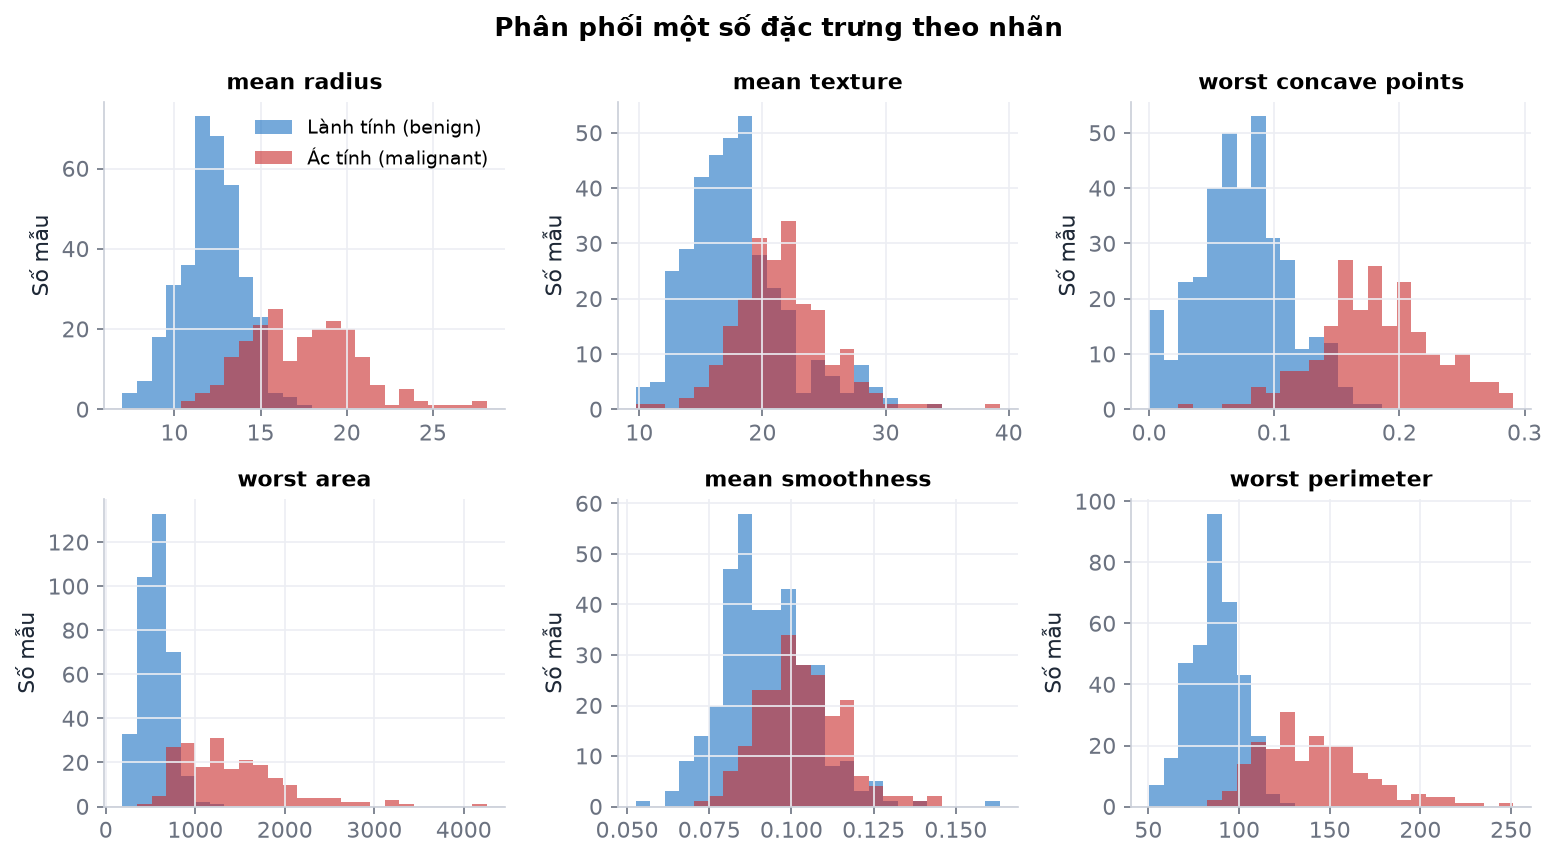
\includegraphics[width=\textwidth]{02_phan_phoi_dac_trung.png}
    \end{column}
  \end{columns}
\end{frame}

\begin{frame}{Kiến trúc tổng thể}
  \centering
  \begin{tikzpicture}[node distance=4mm and 6mm, box/.style={draw, rounded corners, fill=gray!8, minimum height=9mm,
    align=center, font=\small}, >={Stealth[length=2mm]}]
    \node[box] (data) {Dữ liệu};
    \node[box, right=of data] (prep) {Chia 80/20\\ Scaler};
    \node[box, right=of prep] (svm) {SVC RBF\\ GridSearch};
    \node[box, right=of svm] (cal) {Hiệu chỉnh\\+ ngưỡng};
    \node[box, right=of cal] (art) {Artifact\\+ metadata};
    \node[box, below=10mm of art] (api) {FastAPI\\+ UI};
    \node[box, left=of api] (test) {pytest\\+ CI};
    \node[box, left=of test] (gh) {GitHub};
    \node[box, left=of gh] (render) {Render};
    \draw[->] (data) -- (prep); \draw[->] (prep) -- (svm); \draw[->] (svm) -- (cal); \draw[->] (cal) -- (art);
    \draw[->] (art) -- (api); \draw[->] (api) -- (test); \draw[->] (test) -- (gh); \draw[->] (gh) -- (render);
  \end{tikzpicture}
  \vspace{10pt}
  \begin{block}{Nguyên tắc}
    \texttt{StandardScaler} và \texttt{SVC} trong \alert{cùng một Pipeline}, lưu cả pipeline.
    \texttt{train.py} huấn luyện và xuất artifact; \texttt{app/main.py} chỉ nạp và phục vụ.
  \end{block}
\end{frame}

% =============================================================================
\section{Mô hình và huấn luyện}
% =============================================================================

\begin{frame}{SVM rút gọn}
  \begin{itemize}
    \item Lề mềm có trọng số lớp:
      $\displaystyle \min_{\mathbf{w},b,\boldsymbol\xi}\ \tfrac12\lVert\mathbf{w}\rVert^2 + \sum_i C_{y_i}\xi_i$,
      \quad $y_i(\mathbf{w}^\top\phi(\mathbf{x}_i)+b)\ge 1-\xi_i$
    \item \texttt{class\_weight="balanced"}: $C_k = C\cdot\frac{n}{2n_k}$ --- lỗi ở lớp ác tính (ít hơn) bị phạt nặng hơn
    \item Kernel RBF: $K(\mathbf{x},\mathbf{x}') = \exp(-\gamma\lVert\mathbf{x}-\mathbf{x}'\rVert^2)$
    \item Hàm quyết định chỉ phụ thuộc \alert{vector hỗ trợ}:
      $f(\mathbf{x}) = \sum_{i\in\mathcal S}\alpha_i y_i K(\mathbf{x}_i,\mathbf{x}) + b$
    \item SVM cho \emph{điểm}, không cho xác suất $\Rightarrow$ cần \alert{hiệu chỉnh} (Platt / isotonic)
  \end{itemize}
\end{frame}

\begin{frame}{Pipeline và tối ưu siêu tham số}
  \begin{columns}[T]
    \begin{column}{0.46\textwidth}
      \begin{itemize}
        \item 80/20, \texttt{stratify}, \texttt{random\_state=\RandomState}: \NTrain{} train / \NTest{} test
        \item \texttt{GridSearchCV} + \texttt{StratifiedKFold(5)} \alert{chỉ trên train}
        \item $C\in\{0.1, 1, 10, 100\}$, $\gamma\in\{\text{scale}, 0.001, 0.01, 0.1\}$
        \item Chấm bằng \GridScoring
      \end{itemize}
      \vspace{6pt}
      Chọn \textbf{$C=\BestC$, $\gamma=\BestGamma$}: \GridCVMean{} $\pm$ \GridCVStd
    \end{column}
    \begin{column}{0.52\textwidth}
      \centering
      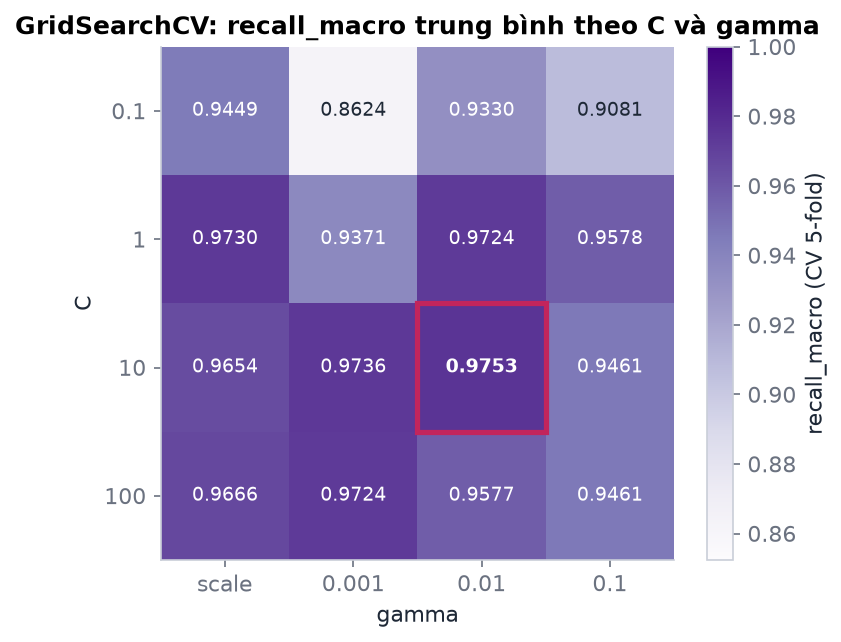
\includegraphics[width=\textwidth]{05_grid_search.png}
    \end{column}
  \end{columns}
\end{frame}

\begin{frame}{Hiệu chỉnh xác suất}
  \begin{columns}[T]
    \begin{column}{0.52\textwidth}
      \centering
      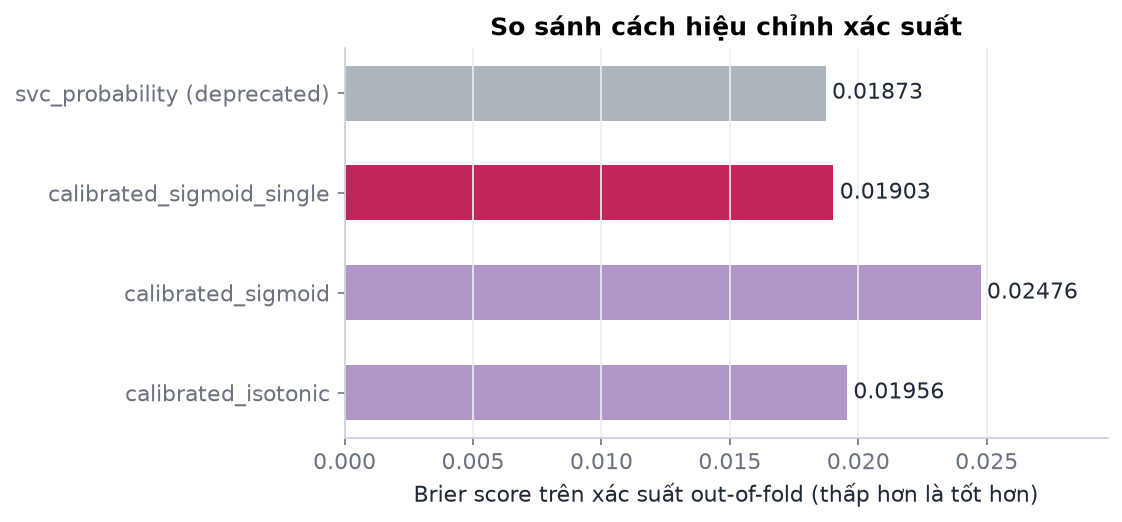
\includegraphics[width=\textwidth]{06_hieu_chinh_xac_suat.png}
    \end{column}
    \begin{column}{0.46\textwidth}
      \small
      \begin{itemize}
        \item So bằng \alert{Brier score} trên xác suất out-of-fold của tập train
        \item \texttt{SVC(probability=True)} thấp nhất (\CalibBaselineBrier) nhưng \alert{deprecated từ scikit-learn 1.9},
              bị xoá ở 1.11
        \item Chọn \CalibChosen{} (\CalibChosenBrier) --- cách scikit-learn khuyên thay thế
      \end{itemize}
    \end{column}
  \end{columns}
\end{frame}

\begin{frame}{Chọn ngưỡng theo sensitivity}
  \begin{columns}[T]
    \begin{column}{0.56\textwidth}
      \centering
      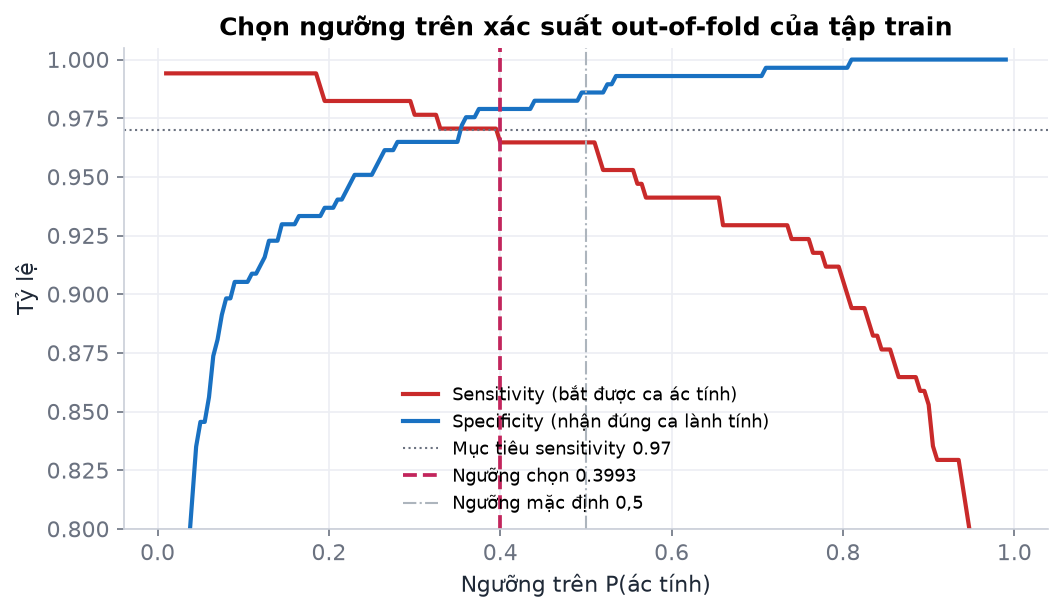
\includegraphics[width=\textwidth]{07_chon_nguong.png}
    \end{column}
    \begin{column}{0.42\textwidth}
      \small
      \begin{itemize}
        \item Ngưỡng \alert{cao nhất} còn giữ sensitivity out-of-fold $\ge \TargetSens$
        \item $\Rightarrow$ \textbf{$t = \Threshold$}; ngưỡng 0,5 chỉ đạt \CVHalfSens
        \item Khoá ngưỡng \alert{trước} khi chạy tập test
        \item API: ác tính nếu $P \ge t$ --- không dùng \texttt{predict()}, nhãn và xác suất luôn nhất quán
      \end{itemize}
    \end{column}
  \end{columns}
\end{frame}

% =============================================================================
\section{Kết quả}
% =============================================================================

\begin{frame}{Kết quả: train · CV · test}
  \begin{columns}[T]
    \begin{column}{0.56\textwidth}
      \footnotesize
      \begin{tabular}{@{}lrrrrr@{}}
        \toprule
        Tập & Sens. & Spec. & Prec. & AUC & FN \\
        \midrule
        \MetricRowsShort
        \bottomrule
      \end{tabular}
      \vspace{8pt}

      \small Test: bắt \textbf{\TestTP/\TestMalignant} ca ác tính, \TestFP{} báo nhầm / \TestBenign{} lành tính.
      Khoảng cách train--CV nhỏ: không quá khớp rõ rệt.
    \end{column}
    \begin{column}{0.42\textwidth}
      \centering
      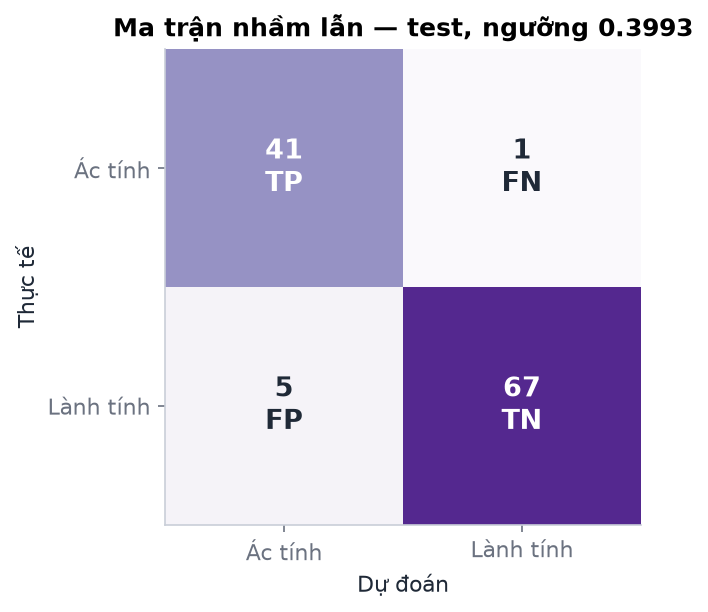
\includegraphics[width=0.92\textwidth]{08_ma_tran_nham_lan.png}
    \end{column}
  \end{columns}
\end{frame}

\begin{frame}{ROC, PR và độ tin cậy của xác suất}
  \begin{columns}[T]
    \begin{column}{0.64\textwidth}
      \centering
      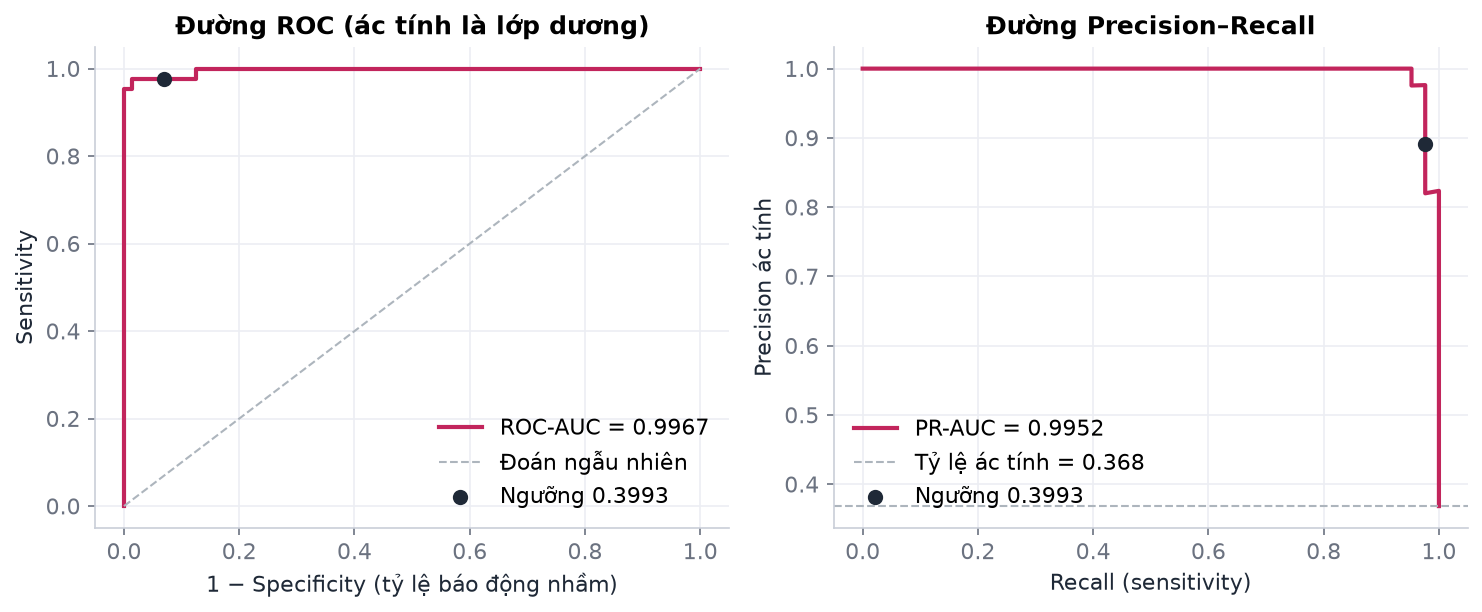
\includegraphics[width=\textwidth]{09_roc_pr.png}
    \end{column}
    \begin{column}{0.34\textwidth}
      \centering
      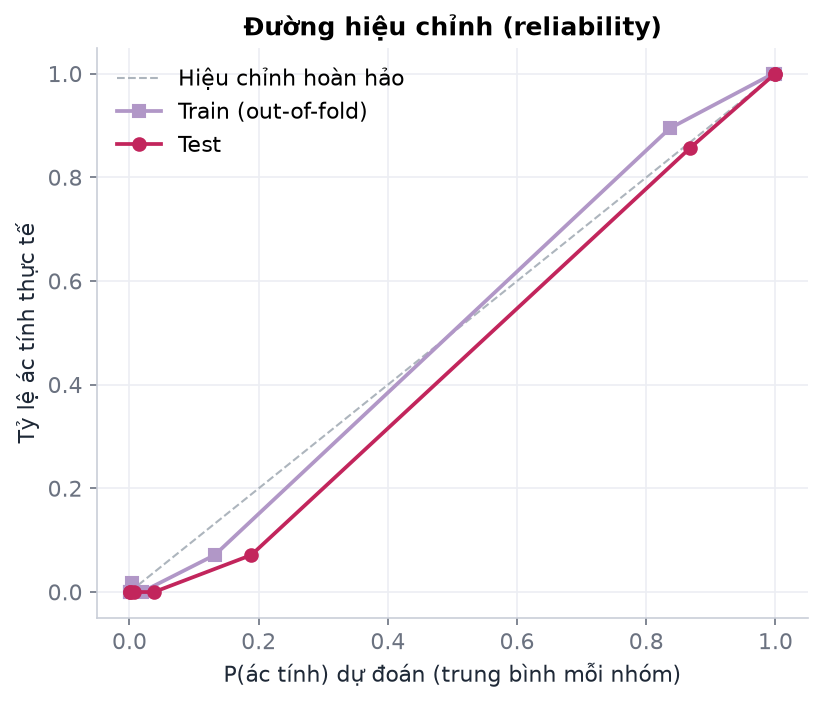
\includegraphics[width=\textwidth]{10_hieu_chinh.png}
    \end{column}
  \end{columns}
  \vspace{4pt}
  \small ROC-AUC \TestAUC, PR-AUC \TestPRAUC, Brier \TestBrier{} trên test; đường hiệu chỉnh bám đường chéo.
\end{frame}

\begin{frame}{Phân tích lỗi --- nhìn thẳng vào ngưỡng}
  \begin{columns}[T]
    \begin{column}{0.5\textwidth}
      \centering
      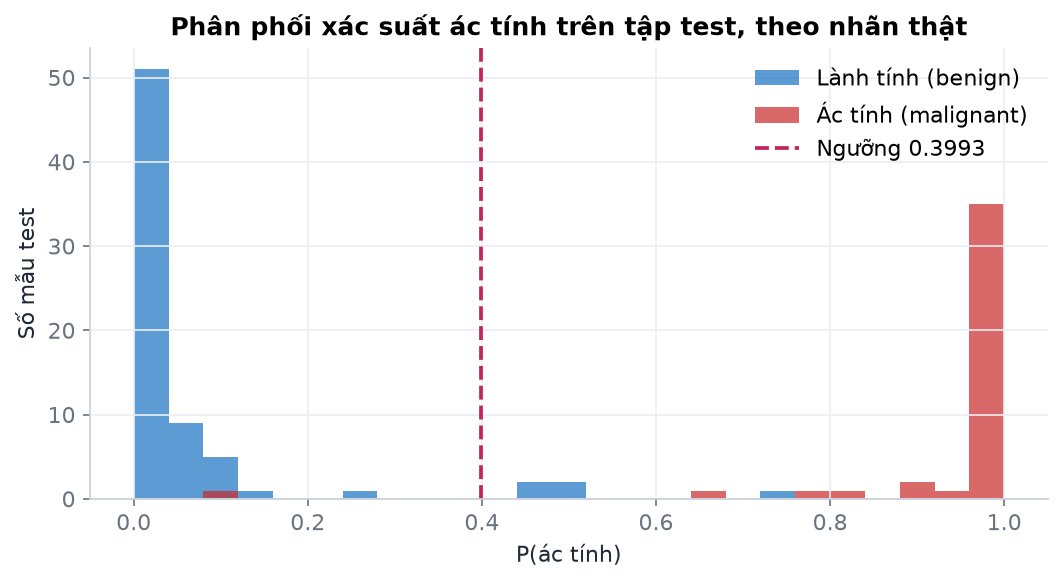
\includegraphics[width=\textwidth]{11_phan_phoi_xac_suat.png}
    \end{column}
    \begin{column}{0.48\textwidth}
      \small
      \begin{itemize}
        \item \TestFN{} ca ác tính bị bỏ sót với $P = \MissedProba$ --- không ngưỡng hợp lý nào bắt được
        \item \TestFP{} ca báo nhầm, \FPBelowHalf{} ca chỉ vì ngưỡng đã hạ
        \item Trên test này, ngưỡng 0,5 cùng sensitivity nhưng ít báo nhầm hơn (\HalfFP)
        \item Nhưng ngưỡng chọn \alert{trên CV}, nơi 0,5 không đạt mục tiêu --- chọn theo test là rò rỉ
      \end{itemize}
    \end{column}
  \end{columns}
\end{frame}

% =============================================================================
\section{API và giao diện}
% =============================================================================

\begin{frame}[fragile]{Thiết kế API}
  \begin{columns}[T]
    \begin{column}{0.5\textwidth}
      \footnotesize
      \begin{tabular}{@{}ll@{}}
        \toprule
        \texttt{GET /health} & 200 / \alert{503} nếu artifact lỗi \\
        \texttt{GET /metadata} & phiên bản, 30 đặc trưng, ngưỡng \\
        \texttt{POST /predict} & 1 bản ghi \\
        \texttt{POST /predict/batch} & 1--100 bản ghi \\
        \texttt{GET /samples} & mẫu test + nhãn thật \\
        \texttt{GET /docs}, \texttt{/ui} & Swagger, giao diện \\
        \bottomrule
      \end{tabular}
    \end{column}
    \begin{column}{0.48\textwidth}
      \small \textbf{422} khi: thiếu / thừa trường (kèm tên), chuỗi, \texttt{null}, NaN, $\infty$, $\le 0$, vượt
      \UpperFactor{}× max tập train
      \vspace{4pt}

      \textbf{Log}: request id, đường dẫn, trạng thái, độ trễ, nhãn --- \alert{không bao giờ} ghi giá trị xét nghiệm
    \end{column}
  \end{columns}
  \vspace{6pt}
\begin{lstlisting}
{"predicted_label": "malignant", "probability_malignant": 0.9971,
 "threshold_malignant": 0.3993, "model_version": "1.0.0", "warning": "..."}
\end{lstlisting}
\end{frame}

\begin{frame}{Giao diện demo}
  \centering
  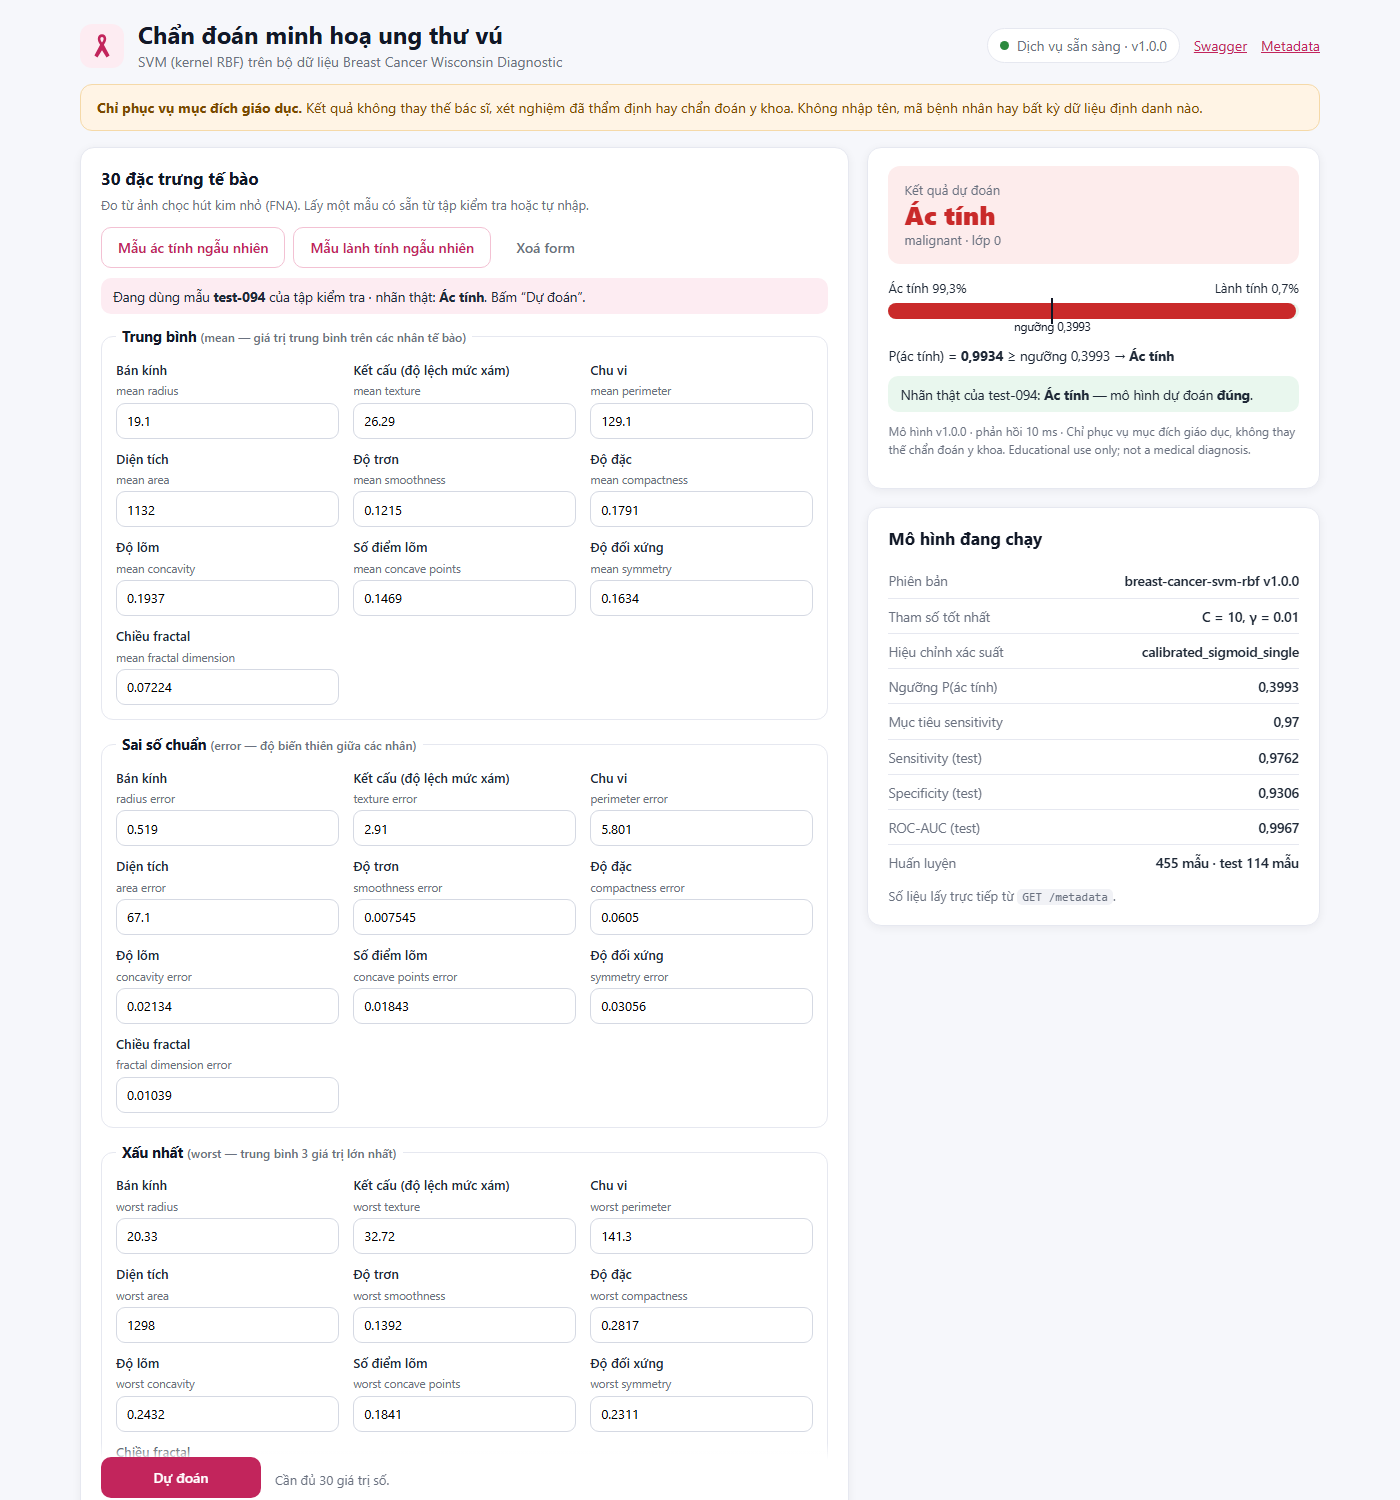
\includegraphics[width=0.86\textwidth]{ui_ac_tinh.png}

  \small Lấy mẫu test ngẫu nhiên · form 30 trường (mean / error / worst) · thanh xác suất có vạch ngưỡng · so với nhãn thật
\end{frame}

% =============================================================================
\section{Kiểm thử và triển khai}
% =============================================================================

\begin{frame}{Kiểm thử và CI}
  \begin{columns}[T]
    \begin{column}{0.5\textwidth}
      \textbf{\texttt{tests/test\_api.py}} --- ma trận của bài giảng
      \small
      \begin{itemize}
        \item Happy path, thiếu / thừa trường
        \item Sai kiểu, NaN, $\pm\infty$, ngoài miền
        \item Batch, samples, 503, request id
        \item Giá trị gửi lên không lọt vào log
      \end{itemize}
    \end{column}
    \begin{column}{0.48\textwidth}
      \textbf{\texttt{tests/test\_model.py}} --- hồi quy mô hình
      \small
      \begin{itemize}
        \item Mẫu cố định $\rightarrow$ nhãn, xác suất cố định
        \item Chỉ số test $\ge$ mức tối thiểu
      \end{itemize}
      \normalsize\textbf{GitHub Actions}
      \small
      \begin{itemize}
        \item ruff $\rightarrow$ pytest $\rightarrow$ \alert{train lại} $\rightarrow$ pytest $\rightarrow$ smoke test
      \end{itemize}
    \end{column}
  \end{columns}
\end{frame}

\begin{frame}[fragile]{Triển khai trên Render}
  \begin{columns}[T]
    \begin{column}{0.5\textwidth}
\begin{lstlisting}
services:
  - type: web
    name: breast-cancer-svm-api
    runtime: python
    buildCommand: pip install -r requirements.txt
    startCommand: uvicorn app.main:app --host 0.0.0.0 --port $PORT
    healthCheckPath: /health
    envVars:
      - key: PYTHON_VERSION
        value: 3.12.10
\end{lstlisting}
    \end{column}
    \begin{column}{0.48\textwidth}
      \small
      \begin{enumerate}
        \item Push GitHub (commit \texttt{artifacts/})
        \item New $\rightarrow$ \textbf{Blueprint} $\rightarrow$ Apply
        \item Health check \texttt{/health} xanh
        \item \texttt{smoke\_test.py <URL>}: 7 bước của bài giảng
      \end{enumerate}
      Phục vụ \alert{đúng artifact đã commit} (không train lúc build); phiên bản thư viện khoá và được kiểm tra khi khởi động.
    \end{column}
  \end{columns}
\end{frame}

\begin{frame}{Bảo mật, giám sát, giới hạn}
  \begin{columns}[T]
    \begin{column}{0.5\textwidth}
      \textbf{Bảo mật và giám sát}
      \small
      \begin{itemize}
        \item HTTPS; không dữ liệu định danh; log không có payload
        \item Theo dõi lỗi HTTP, độ trễ, tỷ lệ nhãn, tần suất ngoài miền (trôi dữ liệu)
        \item Khi có nhãn thật: đánh giá lại sensitivity, hiệu chỉnh
      \end{itemize}
    \end{column}
    \begin{column}{0.48\textwidth}
      \textbf{Giới hạn và hướng phát triển}
      \small
      \begin{itemize}
        \item Một cơ sở, \NSamples{} ca; test chỉ \TestMalignant{} ca ác tính
        \item Chưa kiểm định ngoại bộ; không chia được theo bệnh nhân
        \item Tiếp theo: dữ liệu đa cơ sở, ngưỡng theo chi phí lâm sàng, giải thích dự đoán (SHAP)
      \end{itemize}
    \end{column}
  \end{columns}
\end{frame}

% =============================================================================
\section{Demo và kết luận}
% =============================================================================

\begin{frame}{Demo trực tiếp}
  \begin{columns}[T]
    \begin{column}{0.55\textwidth}
      \begin{enumerate}
        \item Mở \texttt{/ui} $\rightarrow$ \textbf{Mẫu ác tính} $\rightarrow$ Dự đoán
        \item \textbf{Mẫu lành tính} $\rightarrow$ Dự đoán
        \item Xoá một ô $\rightarrow$ gửi qua Swagger $\rightarrow$ \alert{422}
        \item \texttt{/docs}, \texttt{/health}, \texttt{/metadata}
      \end{enumerate}
      \vspace{8pt}
      \small Dịch vụ Free ngủ sau \textasciitilde15 phút: mở trước 1--2 phút
    \end{column}
    \begin{column}{0.43\textwidth}
      \begin{block}{Địa chỉ}
        \centering\small
        \texttt{https://breast-cancer-svm-api-f2qq.onrender.com/ui}
      \end{block}
    \end{column}
  \end{columns}
\end{frame}

\begin{frame}{Kết luận}
  \begin{itemize}
    \item Quy trình đầy đủ: dữ liệu $\rightarrow$ chia tập đúng cách $\rightarrow$ pipeline $\rightarrow$ đánh giá y khoa
          $\rightarrow$ artifact có phiên bản $\rightarrow$ API $\rightarrow$ kiểm thử $\rightarrow$ Render
    \item Test: sensitivity \TestSens, specificity \TestSpec, ROC-AUC \TestAUC{} tại ngưỡng \Threshold{} chọn trước
    \item Bài học: ngưỡng và xác suất quan trọng không kém độ chính xác --- và phải chọn \alert{trước} khi nhìn tập test
  \end{itemize}
  \vfill
  \canhbao
\end{frame}

\begin{frame}[plain]
  \centering
  \vfill
  {\Large Cảm ơn quý vị đã lắng nghe}
  \vspace{12pt}

  \texttt{https://breast-cancer-svm-api-f2qq.onrender.com}
  \vfill
\end{frame}

\end{document}
